\documentclass{article}%
\usepackage[T1]{fontenc}%
\usepackage[utf8]{inputenc}%
\usepackage{lmodern}%
\usepackage{textcomp}%
\usepackage{lastpage}%
\usepackage[head=40pt,margin=0.5in,bottom=0.6in]{geometry}%
\usepackage{graphicx}%
%
\title{\textbf{Caraqueños protestaron por fallas de servicios}}%
\author{JOHANN RANGEL}%
\date{09/10/2018}%
%
\begin{document}%
\normalsize%
\maketitle%
\textbf{URL: }%
http://www.eluniversal.com/caracas/22698/caraquenos{-}protestaron{-}por{-}fallas{-}de{-}servicios\newline%
%
\textbf{Periodico: }%
EU, %
ID: %
22698, %
Seccion: %
caracas\newline%
%
\textbf{Palabras Claves: }%
NO\_TIENE\newline%
%
\textbf{Derecho: }%
2.8, %
Otros Derechos: %
, %
Sub Derechos: %
2.8.1\newline%
%
\textbf{EP: }%
SI\newline%
\newline%
%
\textbf{\textit{En la avenida Francisco de Miranda, frente la calle Lebrún en Petare, municipio Sucre, los vecinos exigieron resolver el suministro de gas doméstico. Igualmente, se registraron acciones de protestas}}%
\newline%
\newline%
%
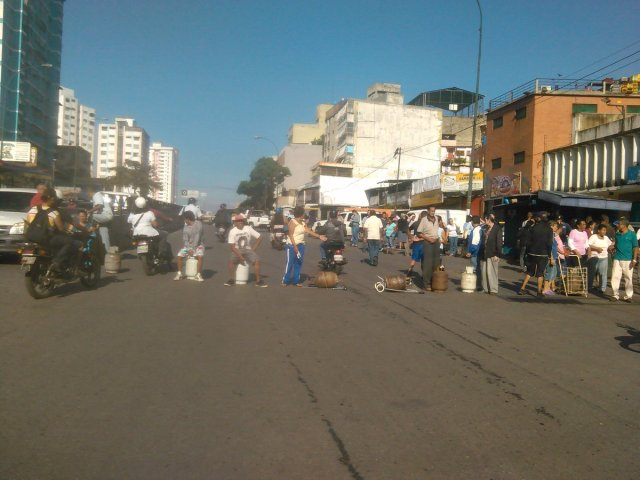
\includegraphics[width=300px]{235.jpg}%
\newline%
%
Caracas.{-}~Un grupo de vecinos  cerró, este lunes, los accesos viales en ambos sentidos en Petare, El Paraíso y San Martín,  para protestar por la falla en  los servicios de gas,  agua y electricidad.%
\newline%
%
En la avenida  Francisco de Miranda, frente la calle Lebrún en Petare, municipio Sucre, los vecinos exigieron resolver el suministro de gas doméstico. \newline%
Igualmente, se registraron acciones de protesta, entre El Paraíso y San Juan, allí una de las vecinas, indicó en una pancarta que no "tienen electricidad desde el pasado 4 de octubre y no tienen agua desde febrero", reportaron usuarios en la red social Twitter.%
\newline%
%
La semana pasada, usuarios en la carretera  Panamericana, reportaron las dificultades para obtener la bombona de gas, por su parte, uno de los usuarios en el oeste de la ciudad, afirmó: "Para poder comprar el gas hay que esperarlo por horas a que llegue. Antes llegaba semanalmente". \newline%
Esta situación  ocurre en los municipios Sucre y Libertador, donde los vecinos deben hacer largas colas para cazar a los camiones de gas comunal, que no tienen días fijos de suministro.%
\newline%
%
Las protestas por el gas se produjeron, este lunes, en otros estados del país, como Táchira, Vargas y Zulia.%
\newline%
%
\end{document}